%!TEX root = main.tex

\section{Index Reduction Algorithm}

\subsection{Separation of Differential and Algebraic Equations}

\begin{frame}{Index Reduction Algorithm}{Separation of Differential and Algebraic Equations}
  \vspace{-1.0em}
  \begin{columns}
    \begin{column}[c]{0.6\textwidth}
      \begin{enumerate}[<+->]
        \item Consider the \textbf{generic} \acsp{DAE} system
        \begin{equation*}
          \mF = \mA \mxp - \mb = \m{0}
        \end{equation*}
        \item \textbf{Separate} the equations with the cokernel $\mK$ and its orthogonal complement $\mN$ of $\mA$
        \begin{equation*}
          \begin{bmatrix} \mE \\ \m{0} \end{bmatrix} \mxp = \begin{bmatrix} \mg \\ \ma \end{bmatrix}
          ~~ \text{with} ~~
          \begin{array}{r@{~}c@{~}l}
            \mE &=& \mN \mA \\
            \mg &=& \mN \mb \\
            \ma &=& \mK \mb
          \end{array}
        \end{equation*}
      \end{enumerate}
      \vspace{-1.0em}
      \uncover<3->{\begin{bbox}[Cokernel Computation]
        The cokernel $\mK$ and its orthogonal complement $\mN$ of $\mA$ are calculated using matrix factorization
      \end{bbox}}
    \end{column}
    \begin{column}[c]{0.4\textwidth}
      \visible<3->{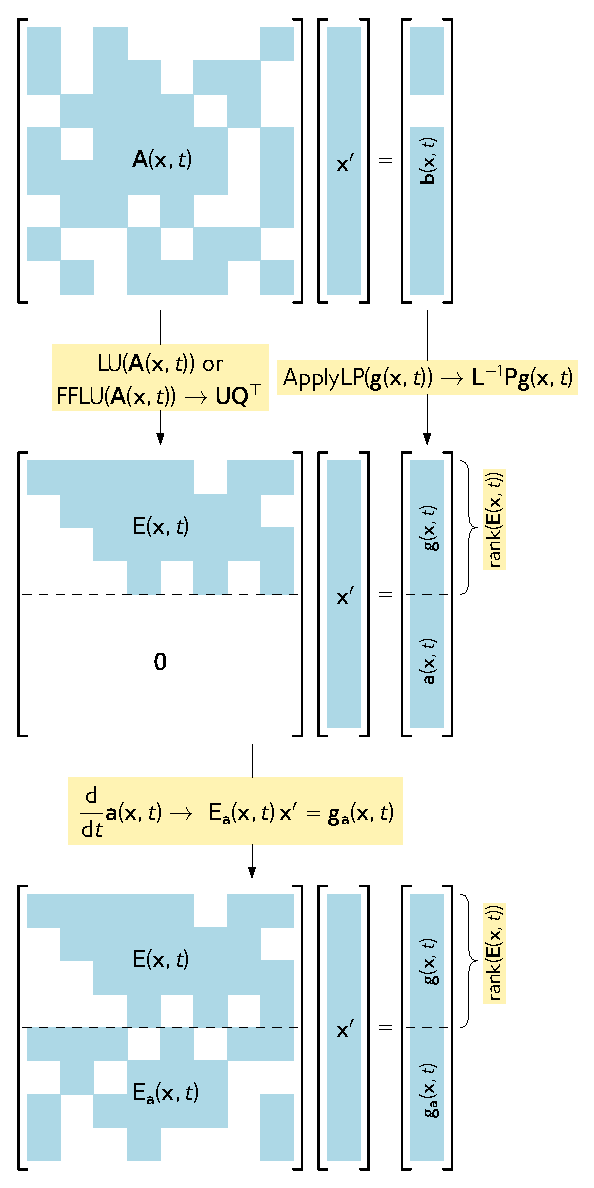
\includegraphics[width=1.0\textwidth, trim={0cm 7.35cm 0cm 0cm}, clip]{dae_visualization.eps}}
    \end{column}
  \end{columns}
\end{frame}

\subsection{Differentiation of Algebraic Equations}

\begin{frame}{Index Reduction Algorithm}{Differentiation of Algebraic Equations}
  \vspace{-1.5em}
  \begin{columns}
    \begin{column}[c]{0.6\textwidth}
      \begin{enumerate}[<+->]\setcounter{enumi}{2}
        \item Update the \textbf{invariants} as $\mh = \mh \cup \ma$
        \item \textbf{Differentiate} the algebraic equations $\ma$
        \begin{equation*}
          \dfrac{\text{d}}{\text{d}t} \ma = \mAd \mxp - \mgd
        \end{equation*}
        \item The \textbf{index reduced} system of \acsp{DAE} takes the form
        \begin{align*}
          \mF = \mA &\mxp - \mb = \m{0} ~~ \text{with} \\
          \mA = \begin{bmatrix} \mE \\ \mAd \end{bmatrix}
          ~~ &\text{and} ~~
          \mb = \begin{bmatrix} \mg \\ \mgd \end{bmatrix}
        \end{align*}
      \end{enumerate}
      \uncover<3->{\begin{bbox}[A Sequential Algorithm]
        Apply \boxednumber{1}--\boxednumber{6} repeatedly until $\mA$ is non-singular
      \end{bbox}}
    \end{column}
    \begin{column}[c]{0.4\textwidth}
      \visible<2->{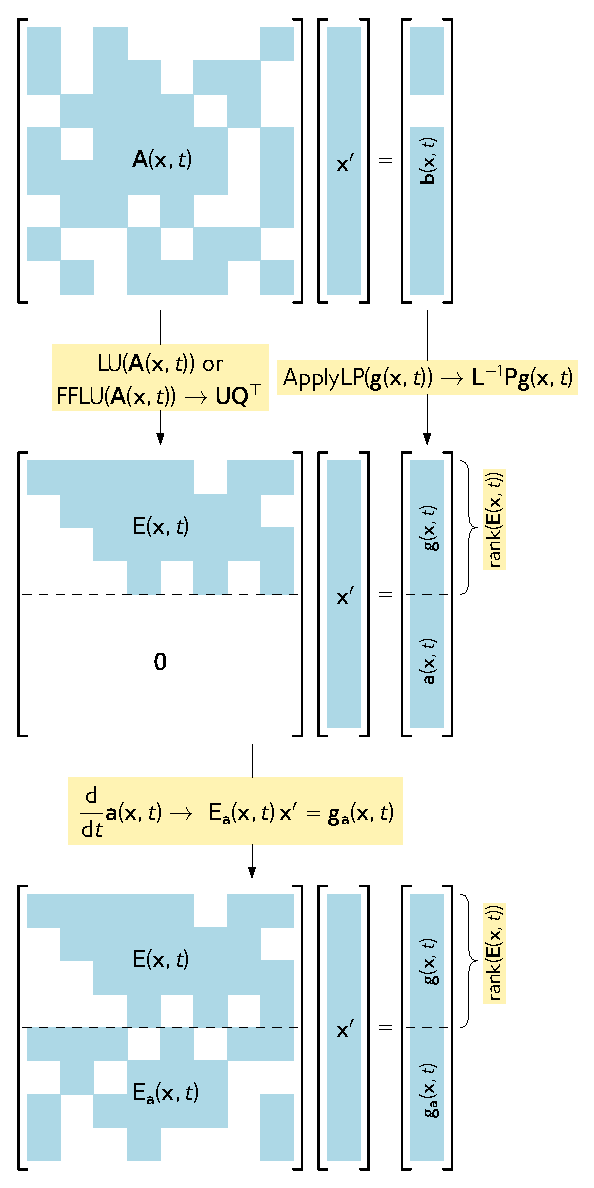
\includegraphics[width=1.0\textwidth, trim={0cm 0cm 0cm 7.35cm}, clip]{dae_visualization.eps}}
    \end{column}
  \end{columns}
\end{frame}

\begin{frame}{Index Reduction Algorithm}{Including Veiling Variables}
  \vspace{-1.0em}
  The algorithm can be extended to include \textbf{\acs{LEM}}
  \begin{itemize}
    \item veiling variables are stored in the list $\mv$
    \item equations are also function of $\mv$
    \item veiling variables add an evaluation layer to the algorithm
  \end{itemize}
  \vspace{-1.5em}\hspace{-0.025\textwidth}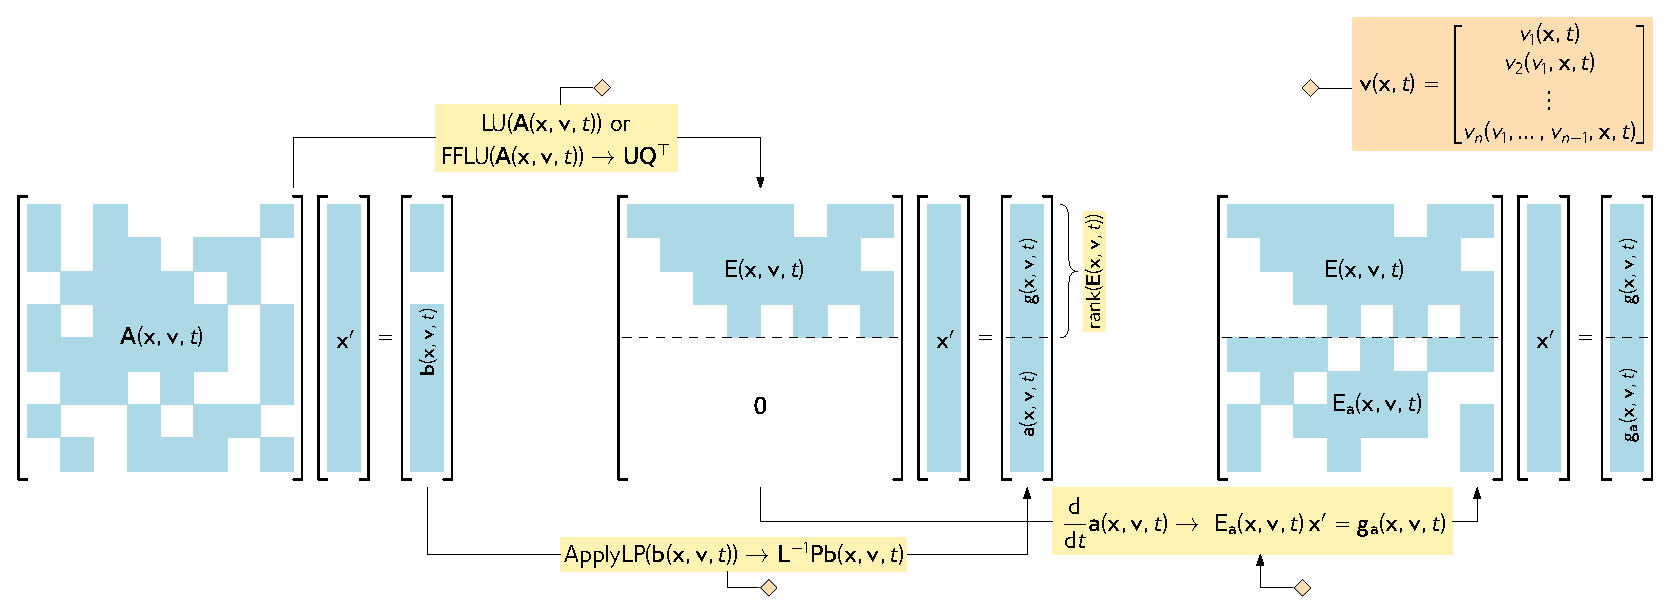
\includegraphics[width=1.05\textwidth]{dae_visualization_veil.eps}
\end{frame}

%\begin{frame}{Index Reduction Algorithm}{Algorithm Flowchart}
%  \centering
%  \begin{tikzpicture}[overlay]
%    \node at (0,0) {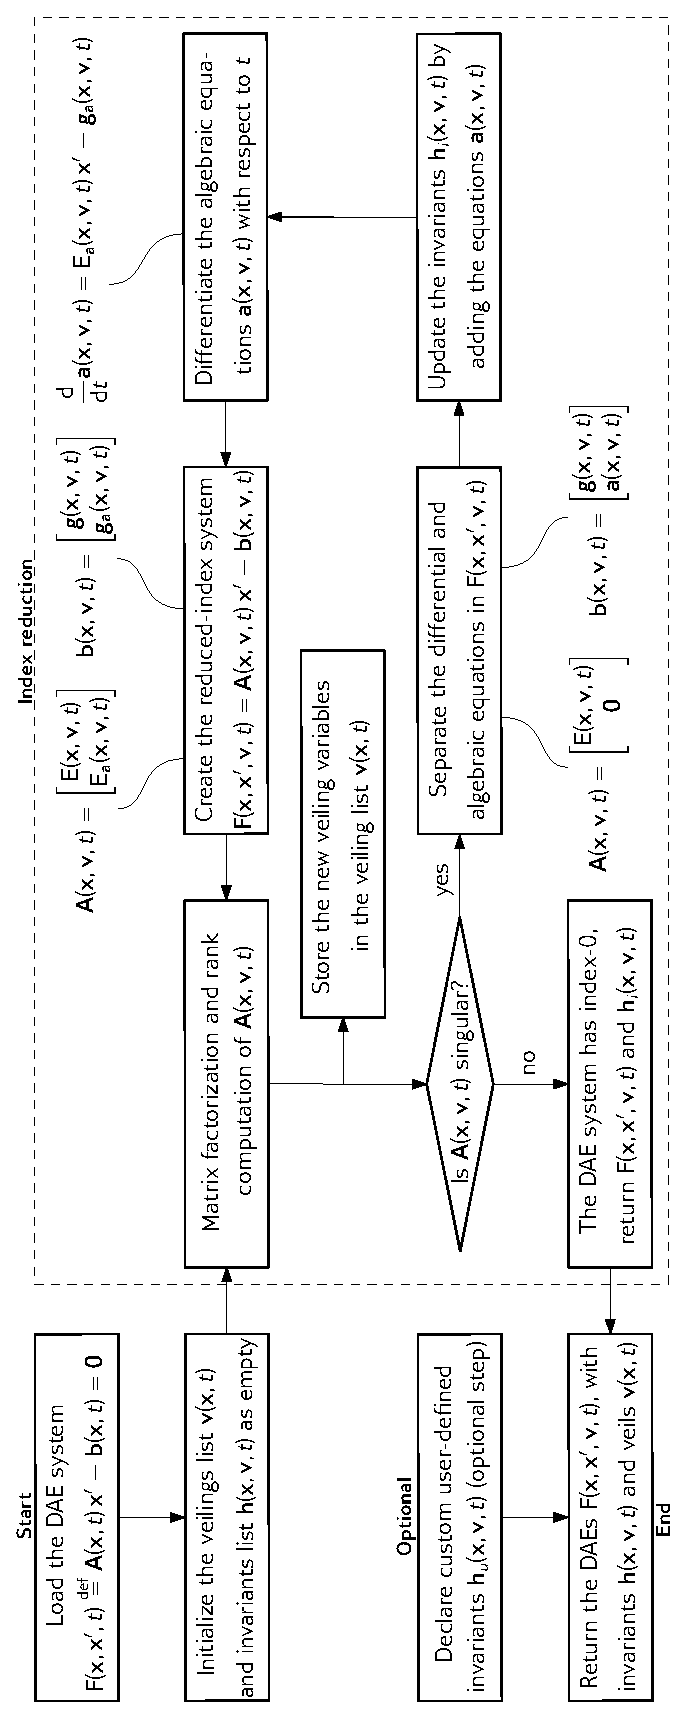
\includegraphics[angle=270, width=1.0\textwidth]{dae_flowchart_veil}};
%    \only<1>{\draw[fg_sl_color, line width=1.0pt] (-7.2,  2.9) rectangle (-3.7,  0.4);} % Initialization
%    \only<2>{\draw[fg_sl_color, line width=1.0pt] (-3.7,  2.9) rectangle ( 7.2, -2.9);} % Index Reduction
%    \only<3>{\draw[fg_sl_color, dashed, line width=1.0pt] (-7.2, -0.3) rectangle (-3.7, -1.6);} % Optional step
%    \only<4>{\draw[fg_sl_color, line width=1.0pt] (-7.2, -1.6) rectangle (-3.7, -2.9);} % Finalization
%  \end{tikzpicture}
%\end{frame}

\begin{frame}{Index Reduction Algorithm}{The Reduced \acs{DAE} System}
  \vspace{-1.0em}
  \hic{\faCanadianMapleLeaf~Now we can code-generate the reduced \acs{DAE} system!}
  \begin{itemize}[<+->]
    \item \textbf{Differential part}
    %
    \begin{equation*}
      \begin{array}{ccl}
          \m{F}(\mx, \mx^\prime, \m{v}, t) = \m{0} & \quad & \text{implicit  system class} \\
          \m{A}(\mx, \m{v}, t) \mx^\prime = \m{b}(\mx, \m{v}, t) & \quad & \text{semi-explicit system class} \\
          \mx^\prime = \m{f}(\mx, \m{v}, t) & \quad & \text{explicit system class}
      \end{array}
    \end{equation*}
    %
    \item \textbf{Invariants}
    %
    \begin{equation*}
      \m{h}(\mx, \m{v}, t) = \begin{bmatrix}
          \mhiv \\
          \mhuv
      \end{bmatrix} = \m{0} \quad \begin{array}{l}
        \text{hidden constraints} \\
        \text{\emph{optional} user-defined invariants}
        \end{array}
    \end{equation*}
    %
    \item \textbf{Veiling variables}
    %
    \begin{equation*}
        \m{v}(\mx, t) = \begin{bmatrix}
            v_{1}(\mx, t) \\
            v_{2}(v_{1}, \mx, t) \\
            \vdots \\
            v_{n}(v_{1}, \dots, v_{n-1}, \mx, t)
        \end{bmatrix}
    \end{equation*}
  \end{itemize}
\end{frame}

\subsection{Projection on Invariants}

\begin{frame}{Projection on Invariants}{Theoretical Background and Implementation}
  \vspace{-1.0em}
  \hic{\faAngleRight\hspace{-0.1em}\faAngleRight\hspace{-0.1em}\faAngleRight~Now we can integrate the system in \Matlab{}!}
  \begin{columns}
    \begin{column}[c]{0.6\textwidth}
      Projection is performed:
      \begin{itemize}
        \item during the \textbf{numerical integration}
        \item to \textbf{enforce} the solution $\mx$ onto the $\mhv$ manifold
        \item by solving the \textbf{constrained minimization} problem
          \begin{align*}
            \underset{\mx}{\text{minimize}} \quad &\dfrac{1}{2}\left(\mx - \tilde{\mx}\right)^2 \\
            \text{subject to} \quad &\mhv = \m{0}
          \end{align*}
        \end{itemize}
      \end{column}
      \begin{column}[c]{0.4\textwidth}
        \hspace{-0.2\textwidth}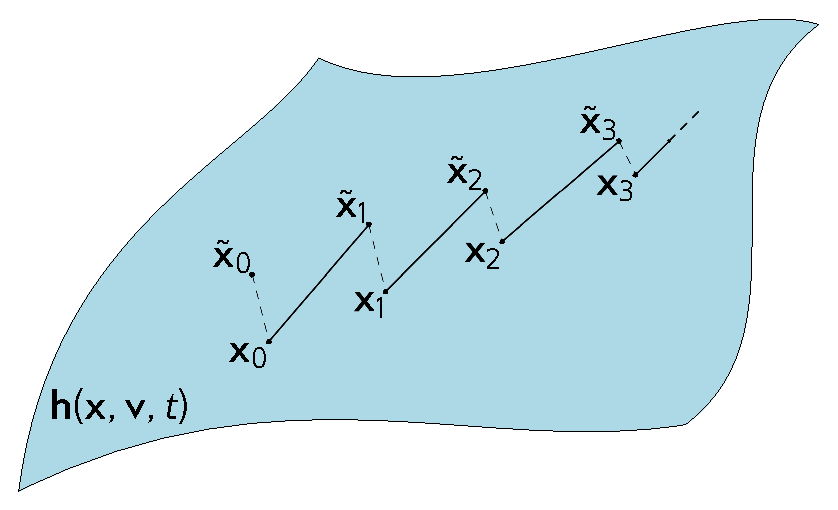
\includegraphics[width=1.2\textwidth]{projection.eps}
      \end{column}
    \end{columns}
    \vspace{1.0em}
    \hic{\large Find $\mx$ with minimal distance from $\tilde{\mx}$ that satisfies the invariants $\mhv$}
\end{frame}

%\begin{frame}{Projection on Invariants}{Theoretical Background and Implementation}
%  \begin{itemize}
%    \item The \textbf{Lagrangian} of the minimization problem is
%    \begin{equation*}
%      \mathcal{L}(\mx, \boldsymbol{\lambda}) = \frac{1}{2}\left(\mx - \tilde{\mx}\right)^2 + \boldsymbol{\lambda} \cdot \mhv
%      \quad \rightarrow \quad
%      \begin{cases}
%        \mx + \m{Jh}_\mx^\top \boldsymbol{\lambda} = \tilde{\mx} \\
%        \mhv = \m{0}
%      \end{cases}
%    \end{equation*}
%    \item The iterative method is \dots
%    \begin{equation*}
%      \begin{bmatrix}
%        \m{Jh}_{\mx} & \m{0} \\
%        \m{I}        & \m{Jh}_\mx^\top
%      \end{bmatrix}
%      \begin{bmatrix}
%        \delta\mx \\
%        \boldsymbol{\lambda}
%      \end{bmatrix} = \begin{bmatrix}
%        \tilde{\mx} - \mx \\
%        -\mhv
%      \end{bmatrix} \quad \text{where the step is} \quad \mx = \tilde{\mx} + \delta\mx
%    \end{equation*}
%    \item[] \dots derived from the \textbf{Taylor expansion}
%    \begin{equation*}
%      \begin{cases}
%        \mhv + \m{Jh}_{\mx}(\mx, \m{v}, t) \delta\mx + \textcolor{mycolor2}{\mathcal{O}\left(\| \delta\mx \|^2\right)} = \m{0} \\
%        \mx + \delta\mx + \m{Jh}_{\mx}^{\top}(\mx + \textcolor{mycolor2}{\delta \mx}, \m{v}, t) \boldsymbol{\lambda} = \tilde{\mx}
%      \end{cases}
%    \end{equation*}
%  \end{itemize}
%\end{frame}

\begin{frame}{Symbolic-Numerical Validation}{The Problem}
  \begin{columns}
    \begin{column}[c]{0.425\textwidth}
      A \textbf{particle} moving over a \textbf{torus} surface
      \begin{equation*}
        \begin{cases}
          x^{\prime}_{1} = u_{1} \\
          x^{\prime}_{2} = u_{2} \\
          x^{\prime}_{3} = u_{3} \\
          u^{\prime}_{1} = u_{3}\cos(t) - x_{3}\sin(t) - u_{2} + 2 c x_{1}\lambda \\
          u^{\prime}_{2} = u_{3}\sin(t) + x_{3}\cos(t) + u_{1} + 2 c x_{2}\lambda \\
          u^{\prime}_{3} = x_{3} + 2x_{3}\lambda \\
          \rho^2 = x_{1}^2 + x_{2}^2 + x_{3}^2 - 2r(x_{1}^2 + x_{2}^2)^{\frac{1}{2}} + r^2
        \end{cases}
      \end{equation*}
      with $c = 1 - r/(x_{1}^2 + x_{2}^2)^{\frac{1}{2}}$, $\rho = 5$, $r = 10$, and ICs $\mx_{0} = [15, 0, 0, 0, 15, -5, \lambda]^{\top}$
    \end{column}
    \begin{column}[c]{0.575\textwidth}
      \hic{\large Exact Solution}
      \begin{equation*}
        \mx_\text{exact} = \begin{bmatrix}
          x_{1} \\ x_{2} \\ x_{3}
        \end{bmatrix} = \begin{bmatrix}
          (\rho \cos(2\pi - t) + r) \cos(t) \\
          (\rho \cos(2\pi - t) + r) \sin(t) \\
          \rho \sin(2\pi - t)
        \end{bmatrix}
      \end{equation*} \\
      \centering{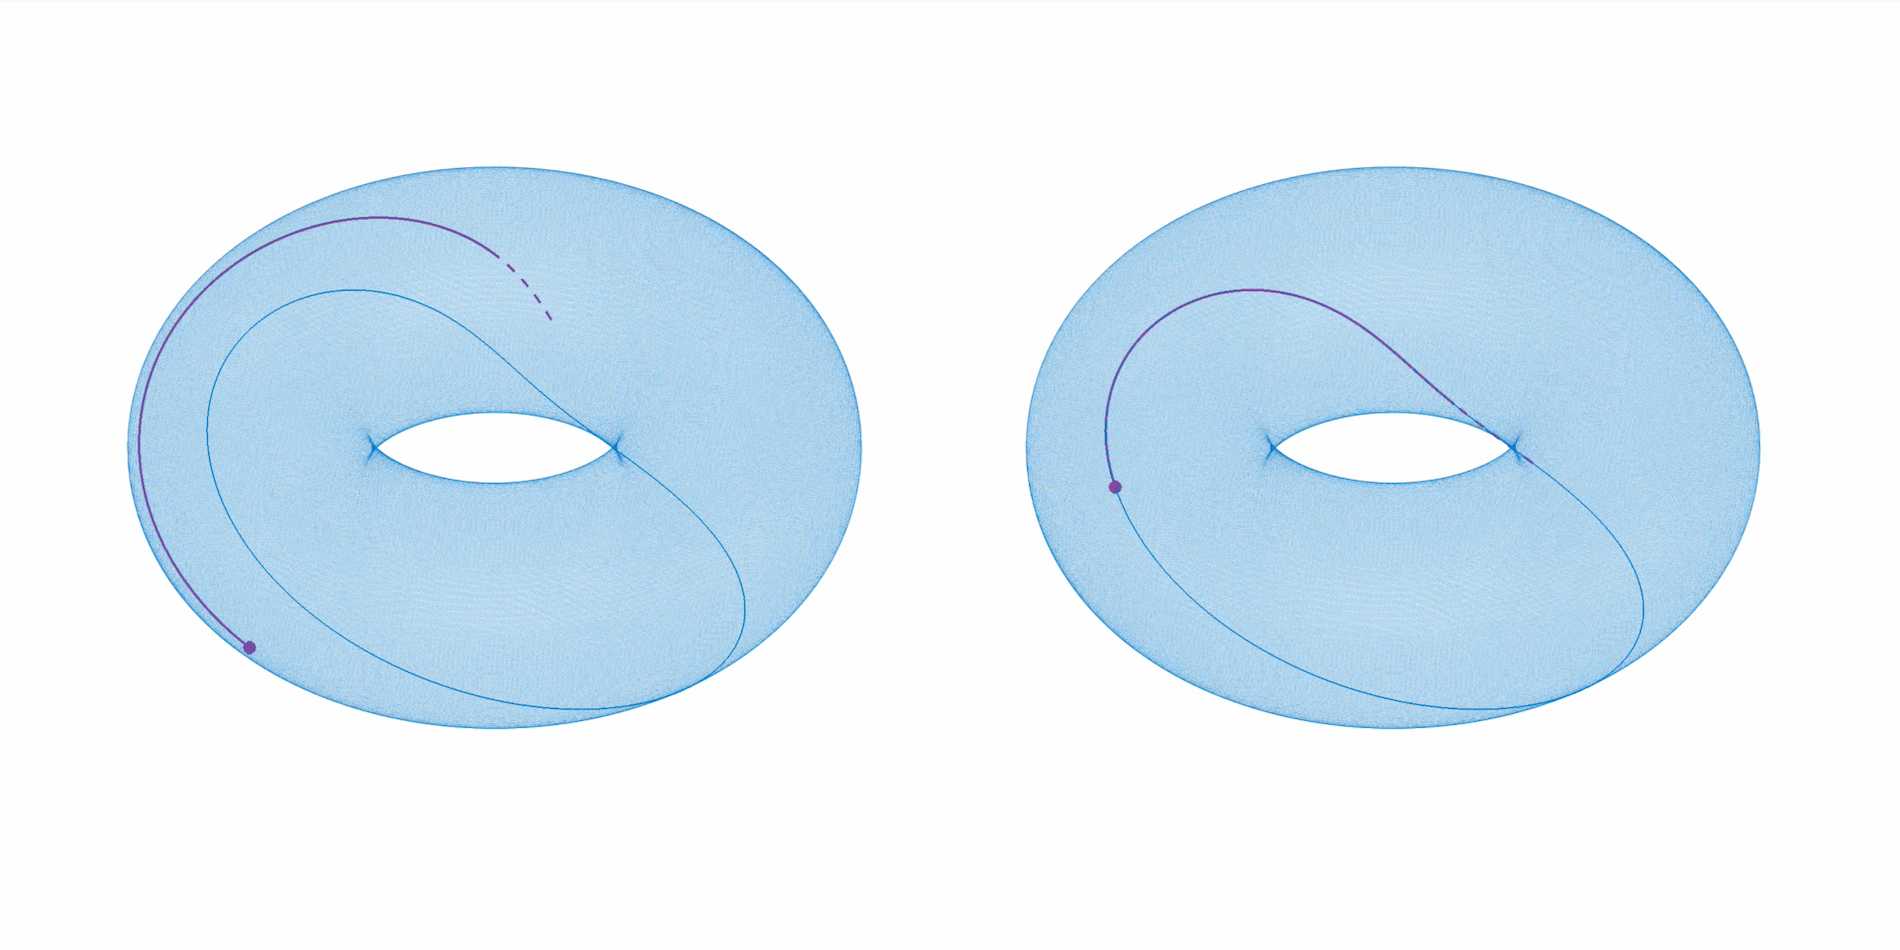
\includegraphics[width=0.6\textwidth, trim={17.0cm 3.5cm 2cm 2.5cm}, clip]{torus_3d_placeholder.png}}
    \end{column}
  \end{columns}
  \vspace{0.5em}
  \scriptsize{\fullcite{campbell1995constraint}}
\end{frame}

\begin{frame}{Symbolic-Numerical Validation}{Index Reduction}
  \vspace{-1.0em}
  \centering{\scriptsize\begin{tabular}{cccc}
    \multicolumn{4}{c}{\textbf{\acs{LU} Factorization}} \\
    \toprule
    \textbf{Original \acsp{DAE}} & \multicolumn{3}{c}{$\mF = 47\cf + 30\cm + 23\ca$ \quad $\mh = 0$} \\
    \midrule
    \textbf{Reduction step} & $\mE$ & $\mg$ & $\ma$ \\
    \midrule
    Index-3 \acsp{DAE} & $0$ & $39\cf + 36\cm + 13\ca$ & $7\cf + 10\cm + 6\ca$ \\
    Index-2 \acsp{DAE} & $0$ & $39\cf + 36\cm + 13\ca$ & $22\cf + 20\cm + 8\ca$ \\
    Index-1 \acsp{DAE} & $0$ & $39\cf + 36\cm + 13\ca$ & $68\cf + 72\cm + 33\ca$ \\
    Index-0 \acsp{DAE} & $388\cf + 424\cm + 180\ca$ & $79\cf + 77\cm + 26\ca$ & $0$ \\
    \midrule
    \rowcolor{mycolor5!25}
    \textbf{Reduced \acsp{DAE}} & \multicolumn{3}{c}{$\mF = 258\cf + 239\cm + 109\ca$ \quad $\mh = 97\cf + 102\cm + 47\ca$} \\
    \bottomrule \\[0.05em]
    %
    \multicolumn{4}{c}{\textbf{\acs{FFLU} Factorization}} \\
    \toprule
    \textbf{Original \acsp{DAE}} & \multicolumn{3}{c}{$\mF = 47\cf + 30\cm + 23\ca$ \quad $\mh = 0$} \\
    \midrule
    \textbf{Reduction step} & $\mE$ & $\mg$ & $\ma$ \\
    \midrule
    Index-3 \acsp{DAE} & $0$ & $39\cf + 36\cm + 13\ca$ & $7\cf + 10\cm + 6\ca$ \\
    Index-2 \acsp{DAE} & $0$ & $39\cf + 36\cm + 13\ca$ & $26\cf + 23\cm + 8\ca$ \\
    Index-1 \acsp{DAE} & $0$ & $39\cf + 36\cm + 13\ca$ & $68\cf + 72\cm + 33\ca$ \\
    Index-0 \acsp{DAE} & $388\cf + 424\cm + 180\ca$ & $79\cf + 77\cm + 26\ca$ & $0$ \\
    \midrule
    \rowcolor{mycolor2!25}
    \textbf{Reduced \acsp{DAE}} & \multicolumn{3}{c}{$\mF = 258\cf + 239\cm + 109\ca$ \quad $\mh = 101\cf + 105\cm + 47\ca$} \\
    \bottomrule \\[0.025em]
    \multicolumn{4}{c}{\small\emph{Legend}: $\cf$ = functions, $\ca$ = additions, $\cm$ = multiplications, and $\cd$ = divisions.}
    \end{tabular}}
\end{frame}

\begin{frame}{Symbolic-Numerical Validation}{Order and Error Analysis}
  \centering{\small{
\begin{tikzpicture}

\begin{axis}[%
  title={Runge-Kutta Methods Order},
  title style={yshift=0.0mm, font=\bfseries},
  minor tick num=1,
  minor grid style={dashed, line width=0.1pt, draw=gray!45},
  major grid style={line width=0.2pt, draw=gray!60},
  width=4.5cm,
  height=4.5cm,
  at={(0.0in,0.0in)},
  scale only axis,
  xmode=log,
  xmin=0.005,
  xmax=0.5,
  xminorticks=true,
  xlabel style={font=\color{black}},
  xlabel={$\Delta t$},
  ymode=log,
  ymin=5.0e-16,
  ymax=20.0,
  yminorticks=true,
  ylabel style={font=\color{black}},
  ylabel={$\varepsilon$},
  axis background/.style={fill=none},
  xmajorgrids,
  xminorgrids,
  ymajorgrids,
  yminorgrids,
  legend style={font=\small, at={(0.97,0.03)}, anchor=south east, legend cell align=left, align=left, draw=black}
]

\addplot[color=mycolor1, line width=0.5pt, mark=*, mark options={fill, scale=0.5, mycolor1}]
  table[row sep=crcr]{%
  0.005 1.879399452620709e-01\\
  0.06 1.711573027753681e+00\\
  0.115 3.063916890081130e+00\\
  0.17 4.231237958056623e+00\\
  0.225 6.302317678343108e+00\\
  0.28 8.762767335676816e+00\\
  0.335 1.028329978855519e+01\\
  0.39 1.252649980402613e+01\\
  0.445 9.207336428245306e+00\\
  0.5 1.299428017259284e+01\\
};
\addlegendentry{Implicit Euler}

\addplot[color=mycolor2, line width=0.5pt, mark=*, mark options={fill, scale=0.5, mycolor2}]
  table[row sep=crcr]{%
  0.005 1.992528035899e-07\\
  0.06 0.000337631444430997\\
  0.115 0.00233186668661123\\
  0.17 0.00737183144006526\\
  0.225 0.0166514146938725\\
  0.28 0.0314018007261607\\
  0.335 0.0510617453643611\\
  0.39 0.0786646899717534\\
  0.445 0.11675270797915\\
  0.5 0.170354895882445\\
};
\addlegendentry{RadauIIA3}

\addplot[color=mycolor4, line width=0.5pt, mark=*, mark options={fill, scale=0.5, mycolor4}]
  table[row sep=crcr]{%
  0.005 6.75015598972095e-14\\
  0.06 1.52360311034272e-08\\
  0.115 3.82347098870639e-07\\
  0.17 2.62977937026676e-06\\
  0.225 1.20705485162631e-05\\
  0.28 3.98898559916816e-05\\
  0.335 0.000112061177007128\\
  0.39 0.000269397467860699\\
  0.445 0.000580087484554959\\
  0.5 0.00113800574884237\\
};
\addlegendentry{RadauIIA5}

\addplot[area legend, draw=none, fill=mycolor1, fill opacity=0.5, forget plot]
  table[row sep=crcr] {%
  x y\\
  0.005 0.187939945262071\\
  0.015 0.187939945262071\\
  0.015 0.494964142080998\\
}--cycle;

\addplot[area legend, draw=none, fill=mycolor2, fill opacity=0.5, forget plot]
  table[row sep=crcr] {%
  x y\\
  0.005 1.992528035899e-07\\
  0.015 1.992528035899e-07\\
  0.015 5.45505603722094e-06\\
}--cycle;

\addplot[area legend, draw=none, fill=mycolor4, fill opacity=0.5, forget plot]
  table[row sep=crcr] {%
  x y\\
  0.005 6.75015598972095e-14\\
  0.015 6.75015598972095e-14\\
  0.015 1.57024270189941e-11\\
}--cycle;

\node[draw, fill=white] at (1.05e-2, 2.00e-02) {\footnotesize{$p = 0.932$}};
\node[draw, fill=white] at (1.05e-2, 2.10e-08) {\footnotesize{$p = 2.958$}};
\node[draw, fill=white] at (1.05e-2, 0.65e-14) {\footnotesize{$p = 5.095$}};
\end{axis}

\begin{axis}[%
  title={Projection Error},
  title style={yshift=0.0mm, font=\bfseries},
  minor tick num=1,
  minor grid style={dashed, line width=0.1pt, draw=gray!45},
  major grid style={line width=0.2pt, draw=gray!60},
  width=4.5cm,
  height=4.5cm,
  at={(7.0cm,0.0in)},
  scale only axis,
  xmin=0,
  xmax=6.28318530717959,
  xlabel style={font=\color{black}},
  xlabel={$t$},
  xlabel shift={0.125em},
  xtick={0, 1.5707963267949, 3.14159265358979, 4.71238898038469, 6.28318530717959},
  xticklabels={$0$, $\pi/2$, $\pi$, $3\pi/2$, $2\pi$},
  %every y tick scale label/.style={
  %  at={(1.015, 0.945)}, anchor=south west, inner sep=0pt
  %},
  ytick scale label code/.code={$\times \, 10^{-13}$},
  ymin=-0.02e-13,
  ymax=1.085e-13,
  ylabel style={font=\color{black}},
  ylabel={$\| \mh \|_{\infty}$},
  %yticklabel pos=right,
  axis background/.style={fill=none},
  xmajorgrids,
  xminorgrids,
  ymajorgrids,
  yminorgrids,
  legend style={font=\small, at={(0.5,0.97)}, anchor=north, legend cell align=left, align=left, draw=black}
]

\addplot[color=mycolor1, line width=0.5pt]
  table[row sep=crcr]{%
  0.0	0\\
  0.06	4.34990500158268e-14\\
  0.12	9.14713630327889e-14\\
  0.18	2.98902106951307e-14\\
  0.24	1.07748232567088e-13\\
  0.3	2.10810383283768e-14\\
  0.36	0\\
  0.42	4.71502785877585e-15\\
  0.48	3.60007915114583e-14\\
  0.54	5.15958404494974e-14\\
  0.6	0\\
  0.66	3.37571546641056e-14\\
  0.72	3.20051218006002e-14\\
  0.78	3.81173776267159e-14\\
  0.84	6.1954391364817e-15\\
  0.9	8.95925122577517e-14\\
  0.96	0\\
  1.02	0\\
  1.08	3.24241260150387e-14\\
  1.14	3.14931663864555e-14\\
  1.2	2.50556225451883e-14\\
  1.26	5.09349295084449e-15\\
  1.32	0\\
  1.38	2.64245779923981e-15\\
  1.44	3.6842072004579e-14\\
  1.5	5.61897690710851e-15\\
  1.56	0\\
  1.62	4.8026106429562e-14\\
  1.68	3.63626524685878e-14\\
  1.74	1.01942880461704e-14\\
  1.8	0\\
  1.86	1.60069355130316e-14\\
  1.92	2.28518820214578e-16\\
  1.98	1.59079989935601e-14\\
  2.04	0\\
  2.1	1.27449819572632e-15\\
  2.16	0\\
  2.22	1.5182461883964e-14\\
  2.28	0\\
  2.34	2.15531930059804e-14\\
  2.4	4.76121391456162e-15\\
  2.46	9.36392103102618e-15\\
  2.52	1.68888906404432e-14\\
  2.58	1.40704033684351e-14\\
  2.64	1.86604175798768e-14\\
  2.7	0\\
  2.76	1.9584060661875e-14\\
  2.82	0\\
  2.88	1.59393949940154e-14\\
  2.94	9.17721100927432e-15\\
  3	7.80968852312227e-15\\
  3.06	7.388064091316e-15\\
  3.12	7.28584971153018e-15\\
  3.18	1.58906318290303e-14\\
  3.24	8.71670113035874e-15\\
  3.3	2.01335164715821e-14\\
  3.36	1.87429669449795e-14\\
  3.42	1.7813725413259e-14\\
  3.48	1.60851063568547e-14\\
  3.54	6.25687551665572e-16\\
  3.6	1.69547170411231e-14\\
  3.66	8.41775766141766e-15\\
  3.72	3.39216511899456e-14\\
  3.78	4.45866709099199e-15\\
  3.84	1.91680683420683e-14\\
  3.9	2.35877773802524e-14\\
  3.96	4.31470535972855e-14\\
  4.02	3.27790567623137e-14\\
  4.08	3.33643422441018e-14\\
  4.14	8.33060192023164e-15\\
  4.2	0\\
  4.26	2.99541085364436e-14\\
  4.32	1.53853495359176e-14\\
  4.38	0\\
  4.44	0\\
  4.5	0\\
  4.56	4.11555718048816e-15\\
  4.62	3.67780794600896e-14\\
  4.68	6.96692544670932e-15\\
  4.74	3.21649541394723e-15\\
  4.8	0\\
  4.86	1.98207634010965e-14\\
  4.92	0\\
  4.98	3.98983227546346e-14\\
  5.04	2.66738145006334e-15\\
  5.1	0\\
  5.16	1.14818597398386e-15\\
  5.22	2.94481485016782e-14\\
  5.28	4.00430584084634e-14\\
  5.34	8.39165155939648e-16\\
  5.4	2.62190029363372e-14\\
  5.46	0\\
  5.52	4.5388851313787e-14\\
  5.58	0\\
  5.64	2.69606312402563e-15\\
  5.7	1.82222934912061e-14\\
  5.76	1.89070359423442e-14\\
  5.82	4.45295027597655e-14\\
  5.88	3.65018441462149e-14\\
  5.94	1.76619003298675e-14\\
  6	4.4664737416553e-14\\
  6.06	3.00820691761593e-14\\
  6.12	4.79911837055461e-14\\
  6.18	1.29969770362389e-14\\
  6.24	8.14452283860879e-14\\
};\addlegendentry{Implicit Euler}

\addplot[color=mycolor2, line width=0.5pt]
  table[row sep=crcr]{%
  0	0\\
  0.06	8.84448873691838e-15\\
  0.12	7.10252993448526e-14\\
  0.18	2.73745627106684e-14\\
  0.24	7.98778880425246e-14\\
  0.3	3.6081075739454e-14\\
  0.36	0\\
  0.42	3.24265476848927e-14\\
  0.48	3.87046037491941e-14\\
  0.54	6.15239311809982e-14\\
  0.6	0\\
  0.66	3.91562582690368e-14\\
  0.72	2.25000036079271e-14\\
  0.78	4.04414271599053e-14\\
  0.84	1.49380061235967e-14\\
  0.9	5.89354034123046e-14\\
  0.96	4.43960827492856e-14\\
  1.02	3.38273659792399e-14\\
  1.08	0\\
  1.14	1.23582540282663e-14\\
  1.2	1.54714760360776e-14\\
  1.26	4.93042497956856e-14\\
  1.32	9.19872936629242e-15\\
  1.38	1.38615479184773e-15\\
  1.44	7.52495018973183e-16\\
  1.5	4.80001254407006e-14\\
  1.56	1.82980829289806e-14\\
  1.62	4.90034281627552e-16\\
  1.68	3.13259870821234e-14\\
  1.74	1.77625688404132e-14\\
  1.8	3.02811591570971e-14\\
  1.86	1.85416404827173e-14\\
  1.92	6.38757726249384e-15\\
  1.98	1.0616430615281e-14\\
  2.04	2.86913740347028e-14\\
  2.1	2.87532747854972e-14\\
  2.16	1.44908645537467e-14\\
  2.22	0\\
  2.28	1.48226453812946e-14\\
  2.34	1.6245848597906e-14\\
  2.4	3.22231789091681e-14\\
  2.46	2.92696331143997e-14\\
  2.52	1.74008700537511e-14\\
  2.58	1.77789685566004e-14\\
  2.64	1.44343986204923e-14\\
  2.7	0\\
  2.76	0\\
  2.82	6.40702877095534e-15\\
  2.88	1.42771571465927e-14\\
  2.94	2.0554256596902e-14\\
  3	7.06195117559697e-15\\
  3.06	0\\
  3.12	7.27089394097636e-15\\
  3.18	4.06350200553687e-14\\
  3.24	3.53559108943528e-16\\
  3.3	1.59074571212465e-14\\
  3.36	6.78088594942458e-15\\
  3.42	0\\
  3.48	0\\
  3.54	6.37313833585726e-15\\
  3.6	2.64233294813674e-14\\
  3.66	9.05705974224811e-15\\
  3.72	9.25806216032326e-15\\
  3.78	2.8421709430404e-14\\
  3.84	0\\
  3.9	3.29455139897558e-14\\
  3.96	1.07330281365035e-14\\
  4.02	0\\
  4.08	2.99993820655985e-14\\
  4.14	2.99302413301819e-14\\
  4.2	8.45649099423198e-15\\
  4.26	0\\
  4.32	2.92414129726747e-14\\
  4.38	1.55071468737394e-14\\
  4.44	2.89702385935865e-14\\
  4.5	3.11590712535806e-14\\
  4.56	8.06643782767062e-15\\
  4.62	3.71860560727394e-14\\
  4.68	1.15774417663157e-14\\
  4.74	2.40000466840985e-15\\
  4.8	7.99747337593166e-16\\
  4.86	2.49901770525562e-14\\
  4.92	6.77554661163664e-15\\
  4.98	1.2538207925704e-14\\
  5.04	3.03245905494408e-14\\
  5.1	2.16408472173715e-15\\
  5.16	1.40062502346563e-14\\
  5.22	3.81524411539504e-14\\
  5.28	3.8071688841407e-14\\
  5.34	1.57202927985259e-14\\
  5.4	3.0377210200149e-14\\
  5.46	7.15590051863223e-14\\
  5.52	4.38239782516872e-14\\
  5.58	1.79951982640777e-14\\
  5.64	6.39867062902223e-14\\
  5.7	6.49615736545083e-14\\
  5.76	1.66177595708798e-14\\
  5.82	1.07695444051526e-13\\
  5.88	0\\
  5.94	3.46718274762021e-14\\
  6	6.08947400862772e-14\\
  6.06	6.27262279676494e-14\\
  6.12	1.05156307287711e-13\\
  6.18	5.75007020364114e-14\\
  6.24	1.72627172653053e-14\\
};
\addlegendentry{RadauIIA3}

\addplot[color=mycolor4, line width=0.5pt]
  table[row sep=crcr]{%
  0	0\\
  0.06	6.71403541230021e-14\\
  0.12	3.77283965133535e-14\\
  0.18	6.34330992622269e-14\\
  0.24	0\\
  0.3	4.65706896752599e-14\\
  0.36	3.53024518099557e-14\\
  0.42	0\\
  0.48	6.01556977798936e-14\\
  0.54	5.6843418860808e-14\\
  0.6	6.3998447010507e-14\\
  0.66	6.89462466735111e-14\\
  0.72	1.11734380999568e-14\\
  0.78	5.84336673739155e-15\\
  0.84	4.51547342643318e-14\\
  0.9	2.40345531292498e-14\\
  0.96	1.35285891842221e-14\\
  1.02	4.89969933702126e-14\\
  1.08	6.44519721994705e-14\\
  1.14	3.82027084757365e-14\\
  1.2	4.63610229041449e-14\\
  1.26	2.14012786085607e-14\\
  1.32	3.62129381964501e-14\\
  1.38	5.14278476238434e-14\\
  1.44	7.52475217963951e-16\\
  1.5	1.51595717211594e-14\\
  1.56	2.01357850117944e-15\\
  1.62	4.90016969470829e-16\\
  1.68	2.15197114109576e-15\\
  1.74	1.42094637215295e-14\\
  1.8	9.14135367252492e-15\\
  1.86	0\\
  1.92	3.33136607299302e-14\\
  1.98	3.83629683826335e-14\\
  2.04	1.59967695360947e-14\\
  2.1	2.94212446823591e-14\\
  2.16	0\\
  2.22	1.51864101443109e-14\\
  2.28	7.27563915445106e-15\\
  2.34	1.93360441784085e-14\\
  2.4	0\\
  2.46	2.9511735315762e-14\\
  2.52	0\\
  2.58	1.77786569080783e-14\\
  2.64	2.85341341331248e-14\\
  2.7	3.06062249475849e-14\\
  2.76	6.05430255954215e-15\\
  2.82	1.35178386471263e-15\\
  2.88	0\\
  2.94	0\\
  3	0\\
  3.06	3.54093358009643e-16\\
  3.12	1.42133513334771e-14\\
  3.18	1.77504779217282e-16\\
  3.24	7.24938179967691e-15\\
  3.3	7.00937076054701e-15\\
  3.36	2.84301825312368e-14\\
  3.42	6.63882013161966e-15\\
  3.48	1.6007712487894e-14\\
  3.54	1.62299374575982e-14\\
  3.6	0\\
  3.66	1.58874434059998e-14\\
  3.72	1.44195741501297e-14\\
  3.78	9.49801118770299e-15\\
  3.84	1.49386437805692e-14\\
  3.9	0\\
  3.96	7.70015247254448e-15\\
  4.02	1.15286998476027e-14\\
  4.08	1.04060301103914e-14\\
  4.14	2.10957320580662e-14\\
  4.2	5.76430753406985e-14\\
  4.26	0\\
  4.32	3.43798720861495e-15\\
  4.38	0\\
  4.44	0\\
  4.5	1.29595646328969e-14\\
  4.56	2.84138752512645e-14\\
  4.62	4.71567077252452e-15\\
  4.68	3.33738140247112e-14\\
  4.74	2.02937095842527e-14\\
  4.8	1.53930076582013e-14\\
  4.86	7.91332496467288e-15\\
  4.92	4.76635995797504e-14\\
  4.98	4.81895564192324e-14\\
  5.04	1.16266826302188e-14\\
  5.1	6.2319428928642e-14\\
  5.16	4.3455302159109e-14\\
  5.22	2.86730496772646e-14\\
  5.28	2.9300964947864e-14\\
  5.34	6.72223560445336e-15\\
  5.4	7.0170982385832e-14\\
  5.46	4.40352521641556e-14\\
  5.52	8.35122710587472e-15\\
  5.58	2.20814842274086e-14\\
  5.64	5.55417576536816e-14\\
  5.7	2.55536510002858e-14\\
  5.76	2.1865754534927e-14\\
  5.82	8.783763173108e-14\\
  5.88	7.96680804218409e-14\\
  5.94	6.22830583836424e-14\\
  6	1.18139987543405e-14\\
  6.06	1.67364446109691e-14\\
  6.12	3.86667246627752e-14\\
  6.18	3.79629193314912e-15\\
  6.24	6.70788729037476e-14\\
};
\addlegendentry{RadauIIA5}

\end{axis}

\end{tikzpicture}%}}
\end{frame}

\begin{frame}{Symbolic-Numerical Validation}{Solution Visualization}
  \vspace{-1.0em}
  \hic{RadauIIA5 \quad $\Delta t = 0.05$\,s \quad $t \in [0, 200\pi]$\,s}
  \vspace{1.0em}
  \centering\small
  \textbf{No projection}%
  \hspace{10.0em}%
  \textbf{With projection}
  \movie[label=show1, width=0.8\textwidth, autostart, poster, showcontrols, loop]{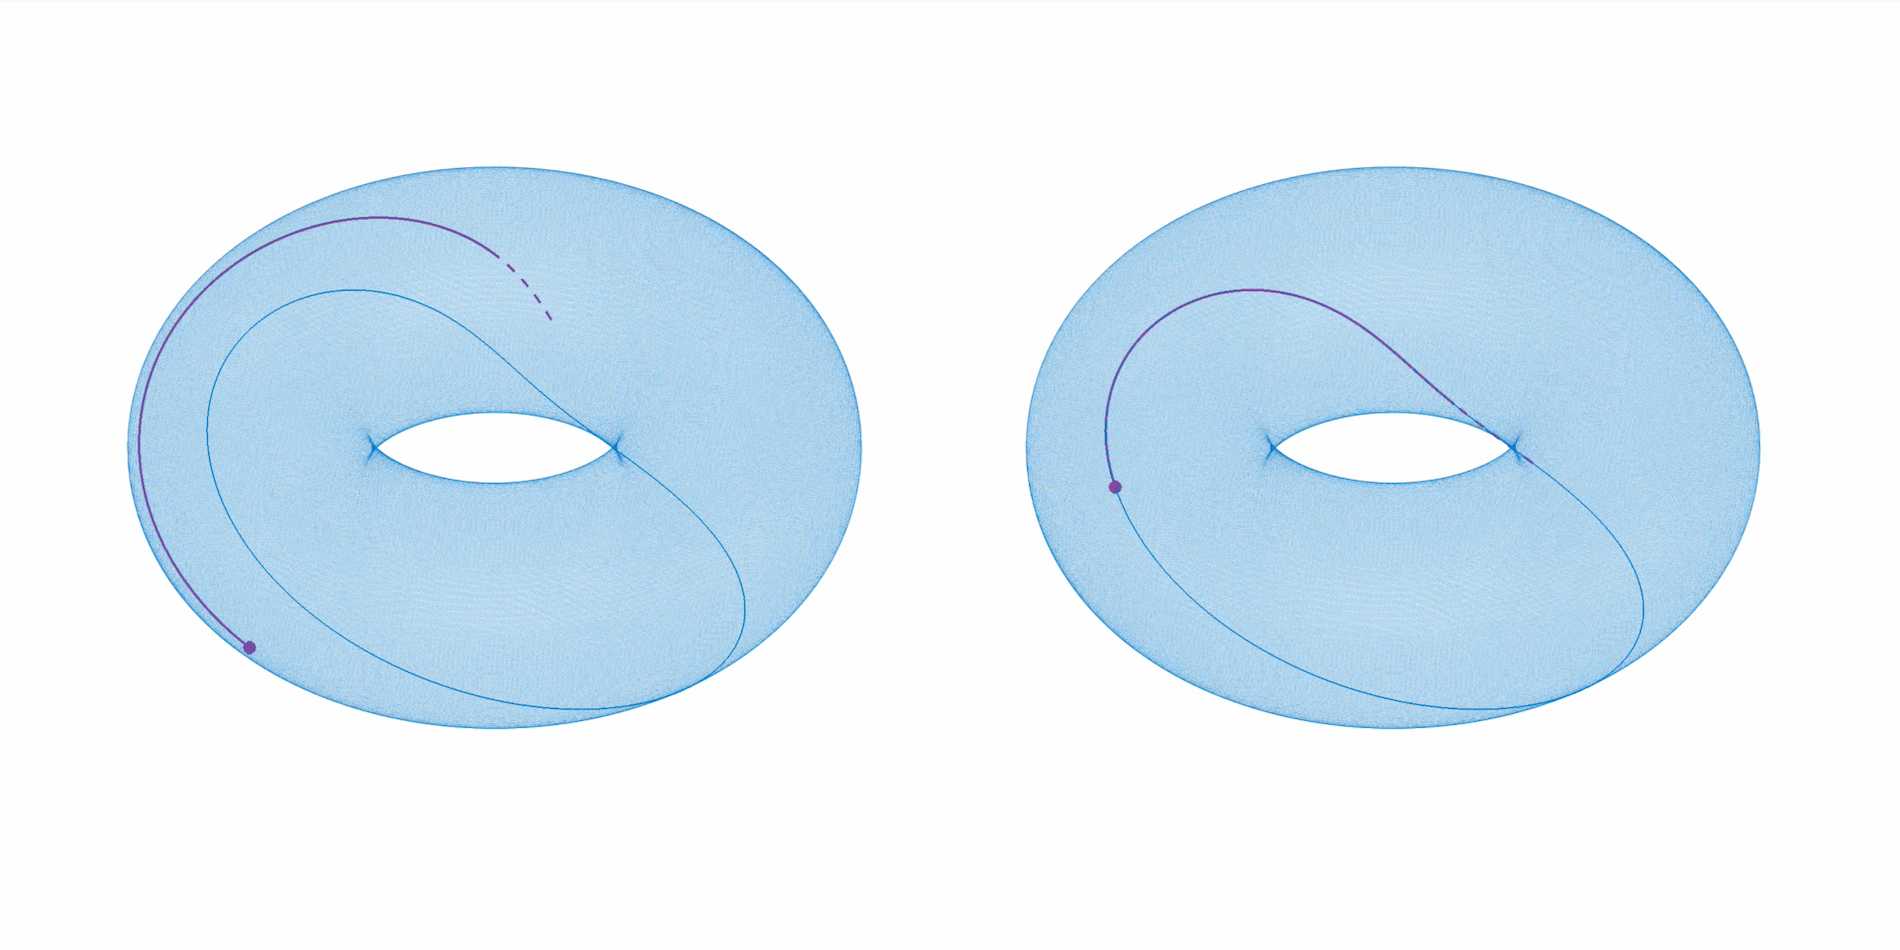
\includegraphics[width=0.8\textwidth]{torus_3d_placeholder.png}}{movie/torus_3d.mov}
\end{frame}

% That's all Folks!